\documentclass[../notas medios.tex]{subfiles}
\begin{document}

\chapter{Análisis de Tensiones}

\graphicspath{{img/Cap3/}} 								 % Specifies the directory where pictures are stored



\subsubsection*{Ejemplo 1: Tracciones sobre un plano arbitrario a partir de $\sigma_{ij}$}
El estado de tensiones sobre un punto material $P$ de un medio continuo está
dado por $\sigma_{ij}$. Determinar el vector de tracciones sobre un plano $T$
definido por los puntos $A$, $B$ y $C$. Adicionalmente determinar las
componentes de la tensión en la dirección normal y paralela al plano.
\subsubsection*{Solución}
Primero necesitamos determinar la ecuación del plano definido por los puntos $A$, $B$ y $C$ y la dirección del vector normal. Recodando que la ecuación del plano esta dada por

\[ax+by+cz=d\]

donde los coeficientes $a$, $b$ y $c$ son las componentes del vector normal $\hat{n}$. Se tiene entonces que:

\[\hat n = \frac{{{{\vec r}_{AC}} \times {{\vec r}_{AB}}}}{{\left\| {{{\vec r}_{AC}} \times {{\vec r}_{AB}}} \right\|}}\]

luego:

\begin{align*}
&a \equiv {n_x}\\
&b \equiv {n_y}\\
&c \equiv {n_z}
\end{align*}

mientras que $d=a x_A+b y_A+c z_A$. Ahora es posible determinar el vector de tracciones sobre una superficie con vector normal $\hat{n}$ usando la \cref{CauchyFormula}:


\[
\left\{ {\begin{array}{*{20}{c}}
{t_x^{(\hat n)}}\\
{t_y^{(\hat n)}}\\
{t_z^{(\hat n)}}
\end{array}} \right\} = \left[ {\begin{array}{*{20}{c}}
{{\sigma _{xx}}}&{{\tau _{xy}}}&{{\tau _{xz}}}\\
{{\tau _{yx}}}&{{\sigma _{yy}}}&{{\tau _{yz}}}\\
{{\tau _{zx}}}&{{\tau _{zy}}}&{{\sigma _{zz}}}
\end{array}} \right]\left\{ {\begin{array}{*{20}{c}}
{{n_x}}\\
{{n_y}}\\
{{n_z}}
\end{array}} \right\}.
\]

Para determinar las componentes normal y paralela se proyecta el vector ${{\vec t}^{(\hat n)}}$ a lo largo de $\hat{n}$. Si se denotan las componentes de ${{\vec t}^{(\hat n)}}$ por $t_x^{(\hat n)}$, $t_y^{(\hat n)}$  y $t_z^{(\hat n)}$  se tiene que:

\[{\sigma _{nn}} = {{\vec t}^{(\hat n)}} \cdot \hat n \equiv t_x^{(\hat n)}{n_x} + t_y^{(\hat n)}{n_y} + t_z^{(\hat n)}{n_z}\]

mientras que la tensión paralela al plano de corte se determina como:

\[\tau _{n\nu }^2 = {{\vec t}^{(\hat n)}} \cdot {{\vec t}^{(\hat n)}} - \sigma _{nn}^2\]



%
\subsubsection*{Ejemplo 2: Círculo de Mohr} 

La \cref{planosEjMohr} muestra dos estados de tensiones para el mismo punto de
un medio continuo. 
%
\begin{figure}[H]
	\centering
		\subfloat [Estado de tensión 1]{ 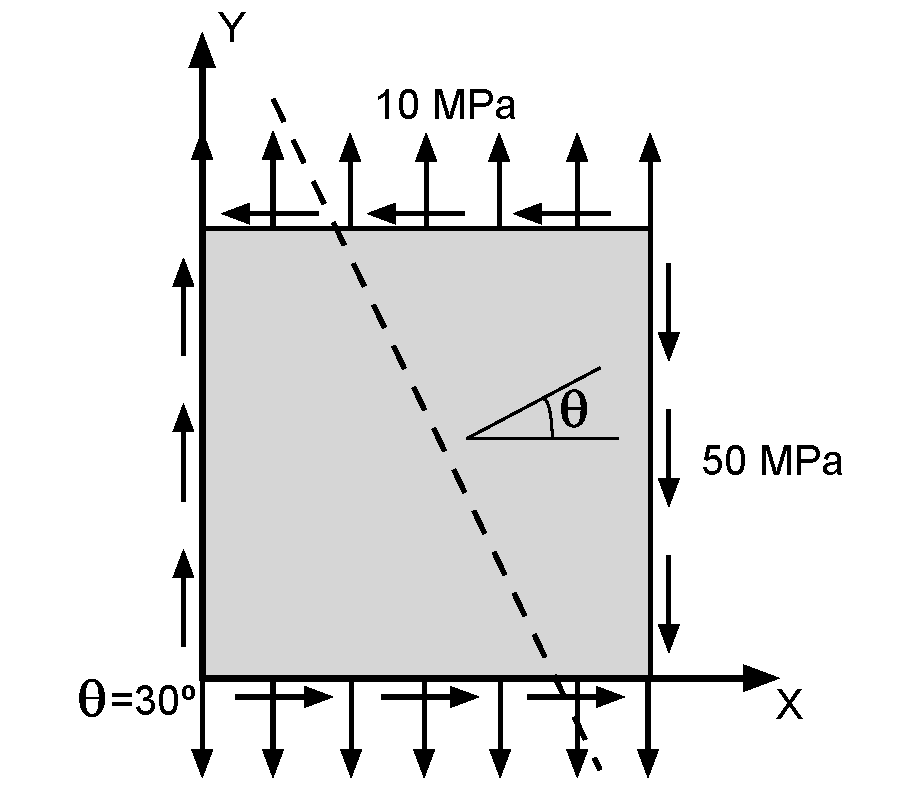
\includegraphics[width=2.8in]{Estado1.pdf}\label{Estado1EjMohr}}
		\hspace{0.5cm}
		\subfloat [Estado de tensión 2]{ 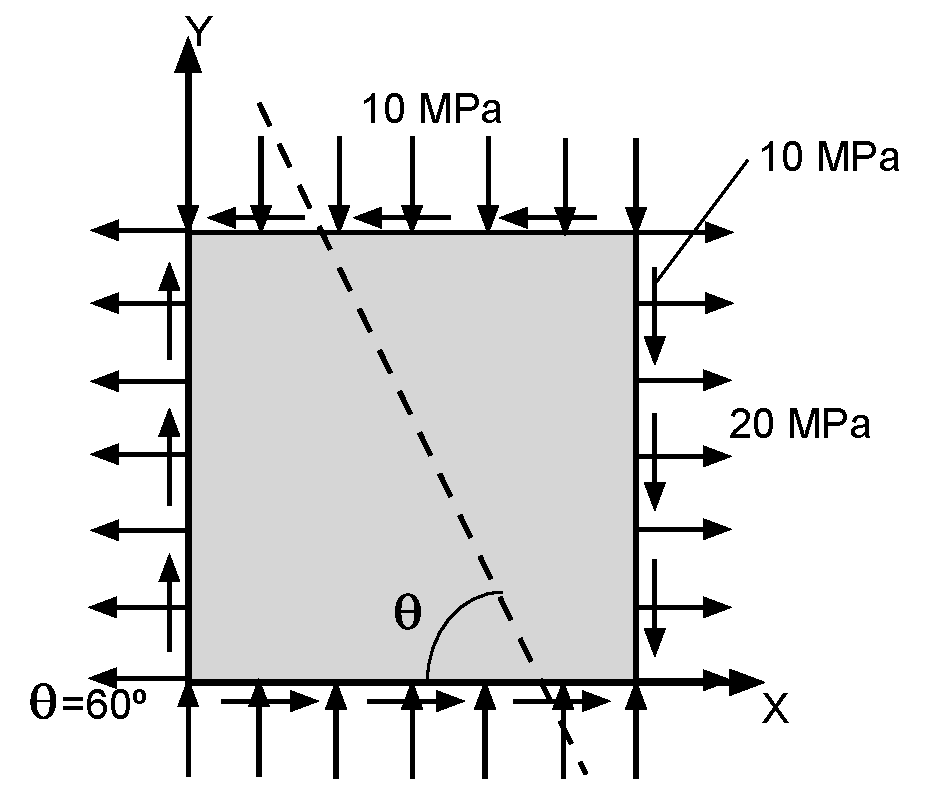
\includegraphics[width=2.8in]{Estado2.pdf}\label{Estado2EjMohr}}		
	\caption{Estado de tensiones en un punto. }
	\label{planosEjMohr}
\end{figure}
%
Para cada estado de carga mostrado en la  \cref{Estado1EjMohr} y en la  \cref{Estado2EjMohr}, respectivamente.
\begin{enumerate}
%
\item[•] Determinar los esfuerzos normales y cortantes sobre los planos mostrados con linea punteada. \\\\
%
\textbf{Solución:}\\\\
%
Inicialmente determinemos el tensor de tensiones para los estados $1$ y $2$
mostrados en la \cref{Estado1EjMohr} y la \cref{Estado2EjMohr} respectivamente.
%
\begin{equation*}
[\sigma_1] =
 	\begin{bmatrix}
     	0.0 & -50.0 & \\
     	-50.0 & 10.0 \\
 	\end{bmatrix}
 \hspace{1cm}
 [\sigma_2] =
 	\begin{bmatrix}
     	20.0 & -10.0 & \\
     	-10.0 & -10.0 \\
 	\end{bmatrix}
\end{equation*}
%
Aunque hay diversos caminos para llegar a una solución, para dar una mayor
ilustración del manejo del círculo de  Mohr haremos uso de esta herramienta
\footnote{Es buen ejercicio cotejar estos resultados haciendo uso del manejo
matricial de la transformación.}. En la  \cref{Tension1} y  en la \cref{Tension2}
se muestra el círculo de Mohr para ambos estados de tensiones. Dicho estado se indica mediante la línea $X-Y$.
%
\begin{figure}[H]
	\centering
		\subfloat [Estado de tensión 1]{ 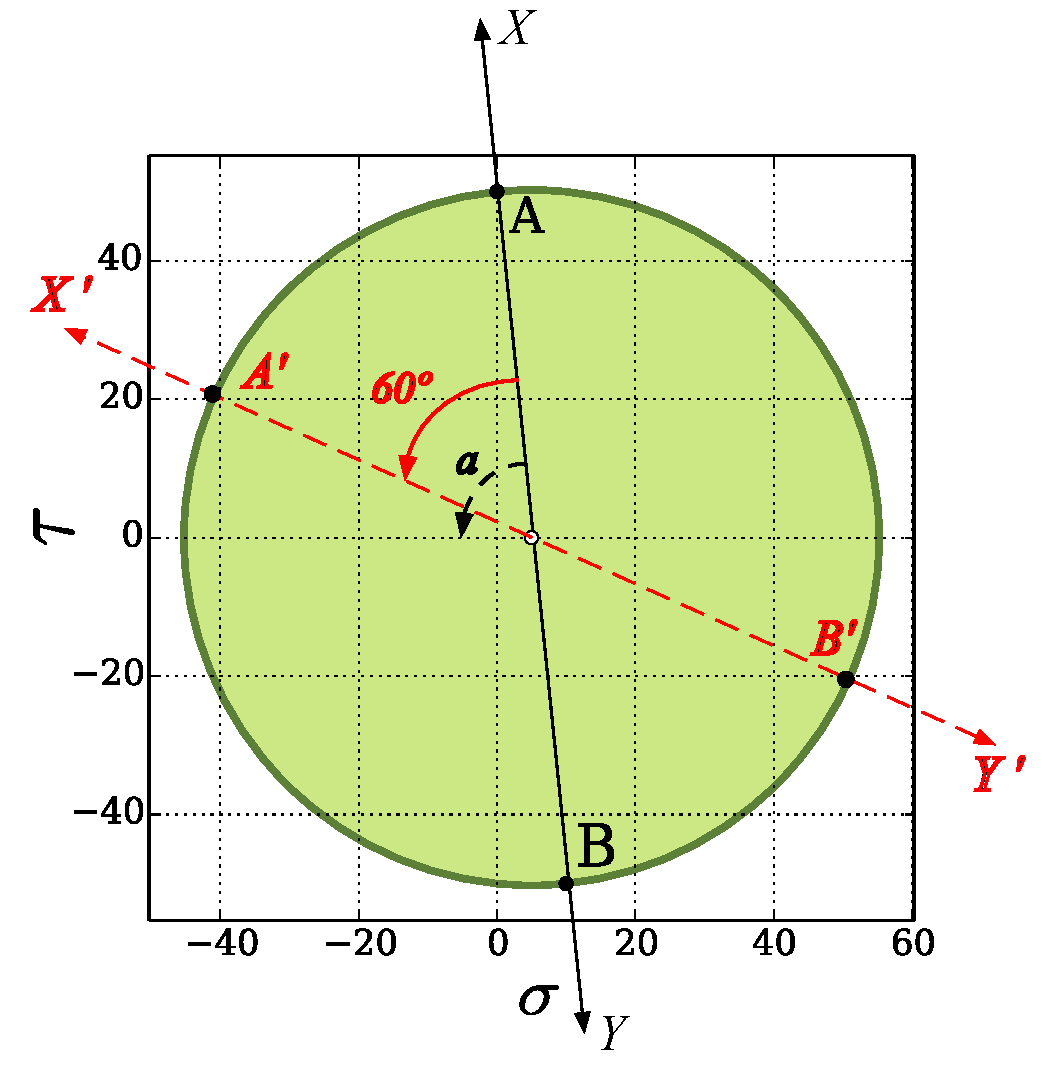
\includegraphics[width=2.8in]{Tensor1.pdf}\label{Tension1}}
		\hspace{0.5cm}
		\subfloat [Estado de tensión 2]{ 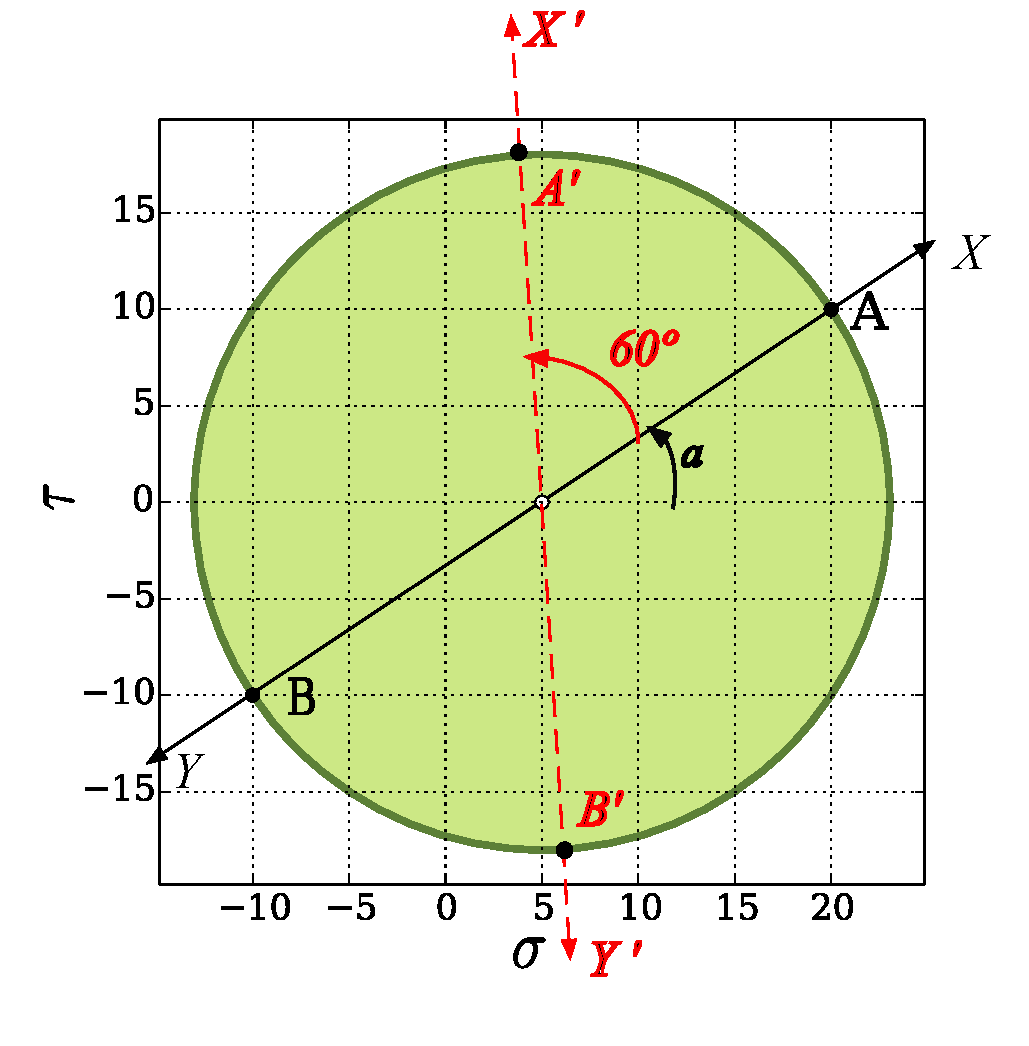
\includegraphics[width=2.8in]{Tensor2.pdf}\label{Tension2}}		
	\caption{Círculo de Mohr con tensor en sistema original $x-y$ y sistema rotado
	$x'-y'$ }
	\label{Tensiones}
\end{figure}
%
Para encontrar las tensiones normales y tangenciales solicitadas hacemos una
rotación de $60^{\circ}$ en el círculo de Mohr ($30^{\circ}$ en el problema
físico) en sentido contrario a las manecillas del reloj. Esta rotación se indica
en el círculo de Mohr de la \cref{Tensiones} mediante las líneas punteadas
color rojo $X'-Y'$ que unen los puntos $A'$ y $B'$. Si se lee la información
de los puntos $A'$ y $B'$ se obtienen los tensores en el sismema $x'-y'$. El
estado de tensiones en el sistema rotado sería entonces dado por:
%
\begin {equation}
\begin {aligned}
 &\tau'_{xy} = R  \sen (\beta) \\
 &\sigma'_{xx} = C - R  \cos(\beta) \\
 &\sigma'_{yy} = C + R  \cos(\beta) \\
\end {aligned}
\label{cicmohr1}
\end {equation}
%
Donde $R$ y $C$ son el radio  y el centro del círculo de Mohr
respectivamente.\\\\
%
Para el estado 1 $R = 50.25$, $C = 5.0$ y $\beta =\alpha - 60 ^{\circ}$. $\alpha
= \arctan\left(\dfrac{50}{5}\right)$ \\
%
Para el estado 2 $R = 18.03 $, $C = 5.0$ y $\beta =180^{\circ} - (\alpha +
60^{\circ})$. $\alpha = \arctan\left(\dfrac{10}{15}\right)$ \\\\
%
Los tensores en el sistema rotado serían: \\
 \begin{equation*}
[\sigma'_1] =
 	\begin{bmatrix}
     	-40.80 & -20.67 & \\
     	-20.67 & 50.80 \\
 	\end{bmatrix}
 \hspace{1cm}
 [\sigma'_2] =
 	\begin{bmatrix}
     	3.83 & -17.99 & \\
     	-17.99 & 6.16 \\
 	\end{bmatrix}
\end{equation*} \\
A partir de los tensores anteriores se concluye que las tensiones normal y tangencial
al plano solicitado son $\sigma=-40.80$ y  $\tau = -20.67$ para el estado $1$ y
$\sigma=3.83$ y  $\tau = -17.99$ para el estado $2$ respectivamente. En la
\cref{Cubo1} y en la \cref{Cubo2} se representa el cubo de tensiones para cada estado.
%

\begin{figure}[H]
	\centering
		\subfloat [Estado de tensión 1]{ 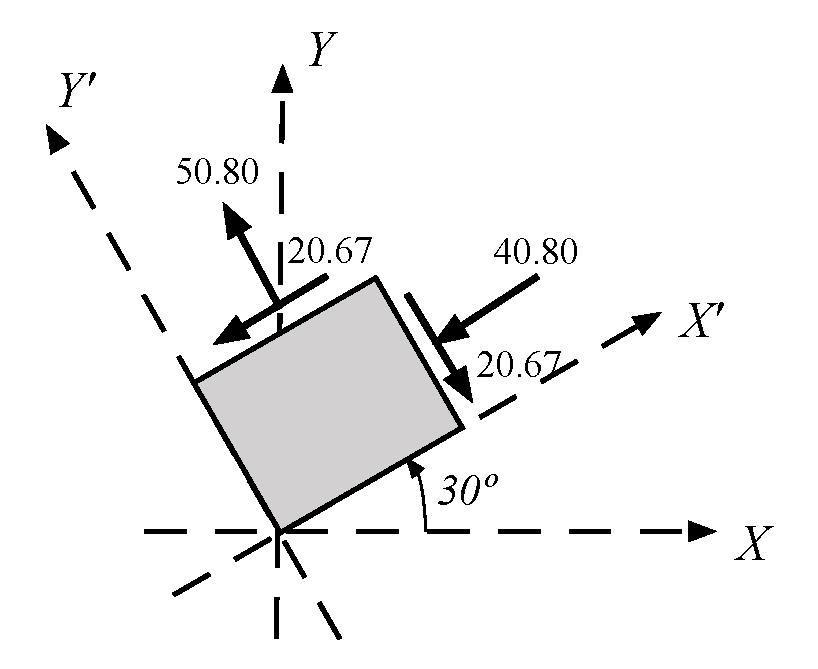
\includegraphics[width=2.8in]{Cubo1.pdf}\label{Cubo1}}
		\hspace{0.5cm}
		\subfloat [Estado de tensión 2]{ 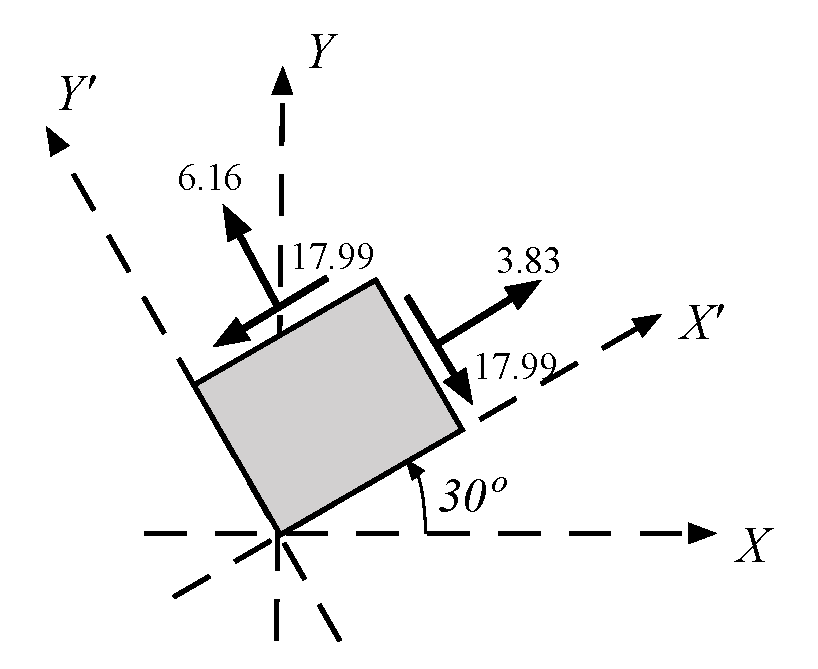
\includegraphics[width=2.8in]{Cubo2.pdf}\label{Cubo2}}		
	\caption{Cubo de Tensiones en sistema rotado $x'-y'$ }
	\label{Cubos}
\end{figure}

%

\item[•] Para cada uno de los estados de tensiones mostrados determinar los valores
propios y las direcciones principales. \\\\
%
\textbf{Solución:}\\\\
%
Los valores principales no son otra cosa que los valores máximos axiales
(normales) a los cuales está sometido el punto. Este estado se logra
precisamente cuando el valor de las tensiones tangenciales es nulo. En la
 \cref{Tens1Prin} y en la  \cref{Tens2Prin} se muestra en el círculo de Mohr, el
sistema original $x-y$ y el sistema principal $x_p - y_p$, mientras que en la \cref{Cubo1Prin} y en la  \cref{Cubo2Prin} se muestra el cubo de tensiones para
el estado principal.


\begin{figure}[H]
	\centering
		\subfloat [Estado de tensión 1]{ 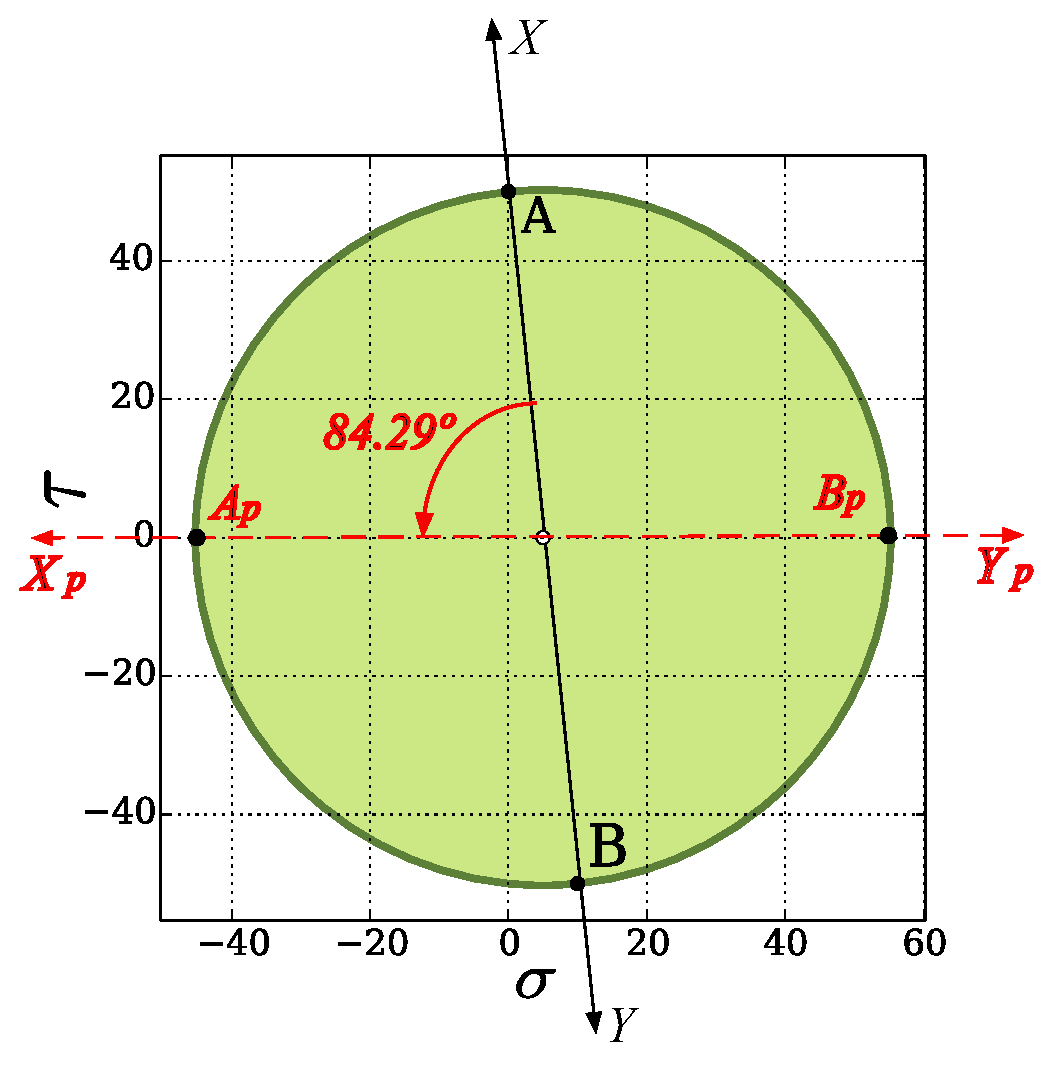
\includegraphics[width=2.8in]{Tens1Prin.pdf}\label{Tens1Prin}}
		\hspace{0.5cm}
		\subfloat [Estado de tensión 2]{ 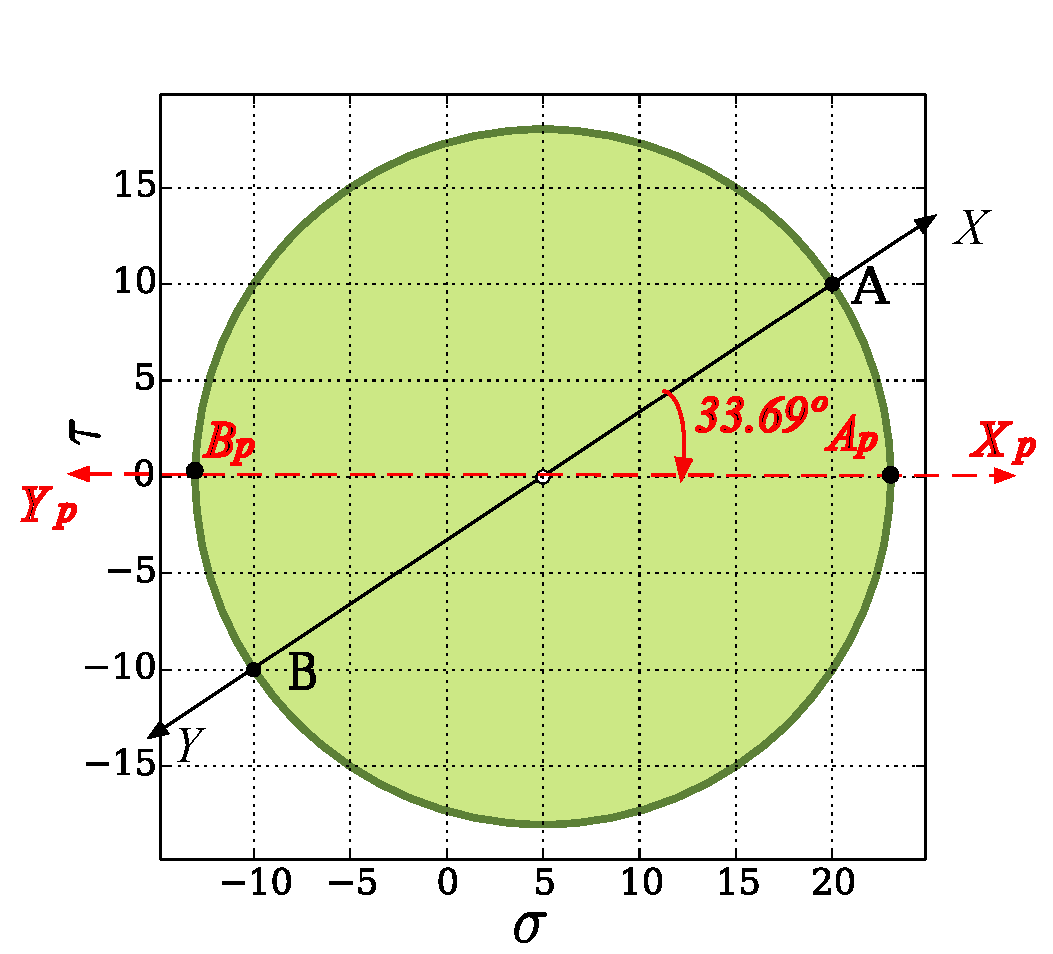
\includegraphics[width=2.8in]{Tens2Prin.pdf}\label{Tens2Prin}}		
	\caption{Círculo de Mohr con valores máximos normales. Puntos $A_p$, $B_p$. }
	\label{TensPrin}
\end{figure}

\begin{figure}[H]
	\centering
		\subfloat [Estado de tensión 1]{ 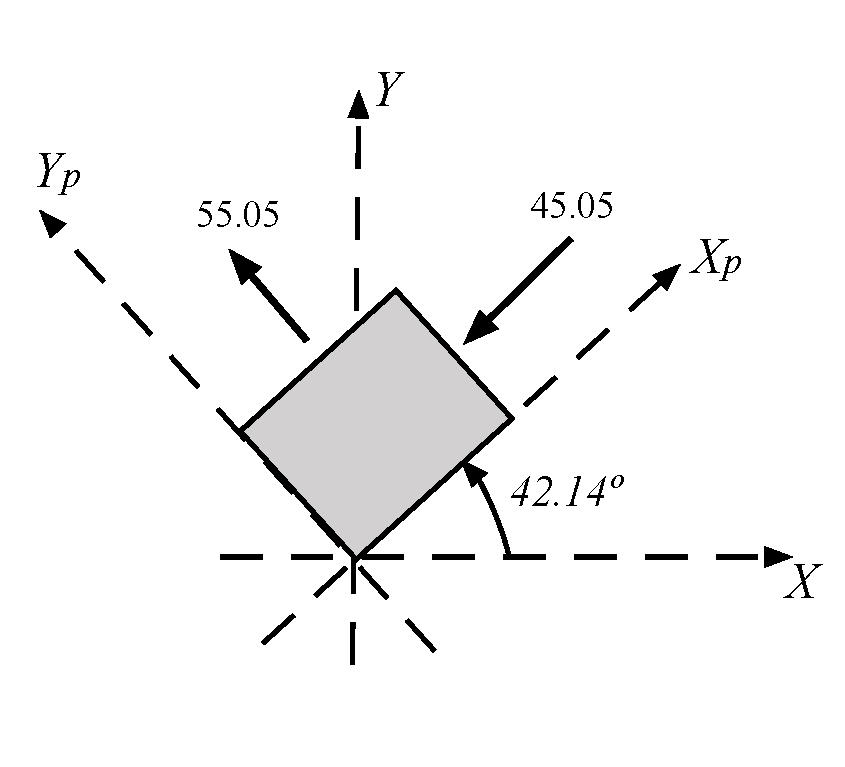
\includegraphics[width=2.8in]{Cubo1Prin.pdf}\label{Cubo1Prin}}
		\hspace{0.5cm}
		\subfloat [Estado de tensión 2]{ 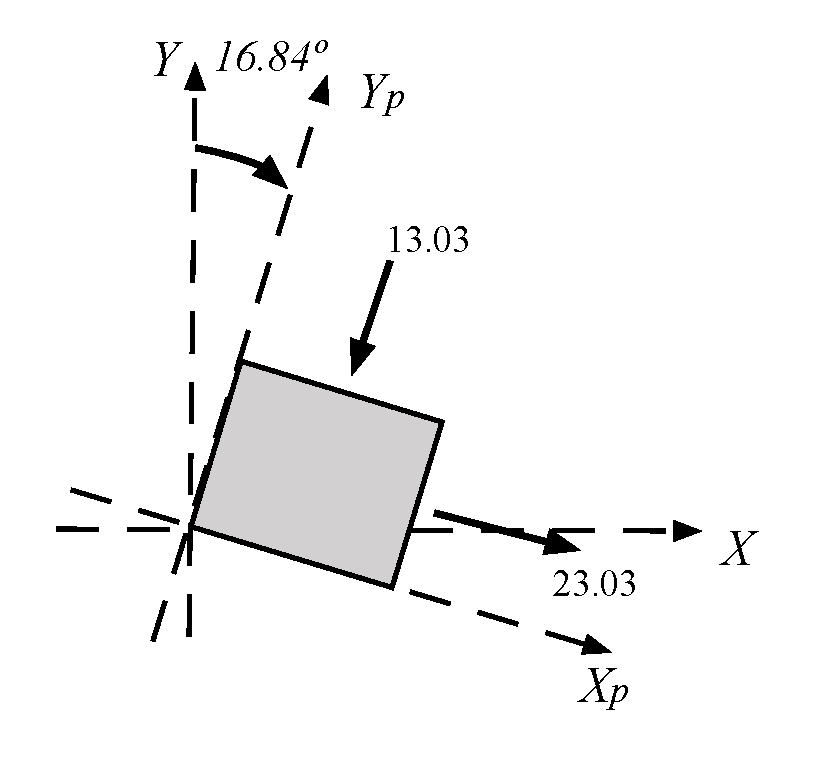
\includegraphics[width=2.8in]{Cubo2Prin.pdf}\label{Cubo2Prin}}		
	\caption{Cubo de tensiones en sistema rotado $x_p-y_p$. }
	\label{CubosPrincipal}
\end{figure}

%
%
%
Nótese que para encontrar el estado principal $1$ rotamos desde el sistema
original $xy$ un ángulo $\alpha = \arctan\left(\dfrac{50}{5}\right)$ en sentido
contrario a las manecillas del reloj, mientras que para el estado principal $2$
rotamos un ángulo $\alpha = \arctan\left(\dfrac{10}{15}\right)$ en sentido de
las manecillas \footnote{La rotación puede ser hecha en cualquier sentido; lo
importante es no perder de vista la ubicación de los ejes y tener en cuenta
que estas rotaciones coinciden en sentido con el problema físico pero que
corresponden a valores de ángulo doble en el círculo}.
Por similitud a la  \cref{cicmohr1} las ecuaciones para encontrar los valores se podrían escribir como:\\
%
\begin {equation}
\begin {aligned}
&\tau^p_{xy} = R \\
&\sigma^p_{xx} = C \pm R \\
&\sigma^p_{yy} = C \mp R  \\
\end {aligned}
\label{cicmohr2}
\end {equation}
%
Los estados de tensiones principales quedarían escritos como:\\
%
 \begin{equation}
[\sigma^p_{1}] =
 	\begin{bmatrix}
     	-45.25 & 0.0 &  \\
     	0.0 & 55.25 \\
 	\end{bmatrix}
 \hspace{1cm}
 [\sigma^p_{2}] =
 	\begin{bmatrix}
     	23.03 & 0.0 &  \\
     	0.0 & -13.03 \\
 	\end{bmatrix}
\end{equation}
%

%
\item[•] Asuma que ambos estados de tensiones ocurren al mismo tiempo y determine
las direcciones principales y valores propios para el estado de tensiones
resultantes. \\\\
%
\textbf{Solución:}
%
Para hacer superposición de los estados de tensiones ambos deben de estar en el
mismo sistema de referencia. En nuestro caso se tiene que inicialemente ambos
están escritos en el mismo sistema de referencia $x y$, por lo que bastará hacer
la suma componente a componente de ambos tensores.
\begin{equation}
[\sigma_t] =
 	\begin{bmatrix}
     	0.0 & -50.0 &  \\
     	-50.0 & 10.0 \\
 	\end{bmatrix}
	+
 	\begin{bmatrix}
     	20.0 & -10.0 &  \\
     	-10.0 & -10.0 \\
 	\end{bmatrix}
 	=
 	\begin{bmatrix}
     	20.0 & -60.0 &  \\
     	-60.0 & 0.0 \\
 	\end{bmatrix}
\end{equation}
%
En la  \cref{TensorSup} se presenta el círculo de Mohr
con el estado original producto de la superposición (linea $X -Y$) y el estado
principal (linea $X_p - Y_p$) mientras que en la \cref{CuboSup} se muestra
el cubo de tensiones del estado principal.
%
\begin{figure}[H]
	\centering
		\subfloat [Circulo de Mohr]{ 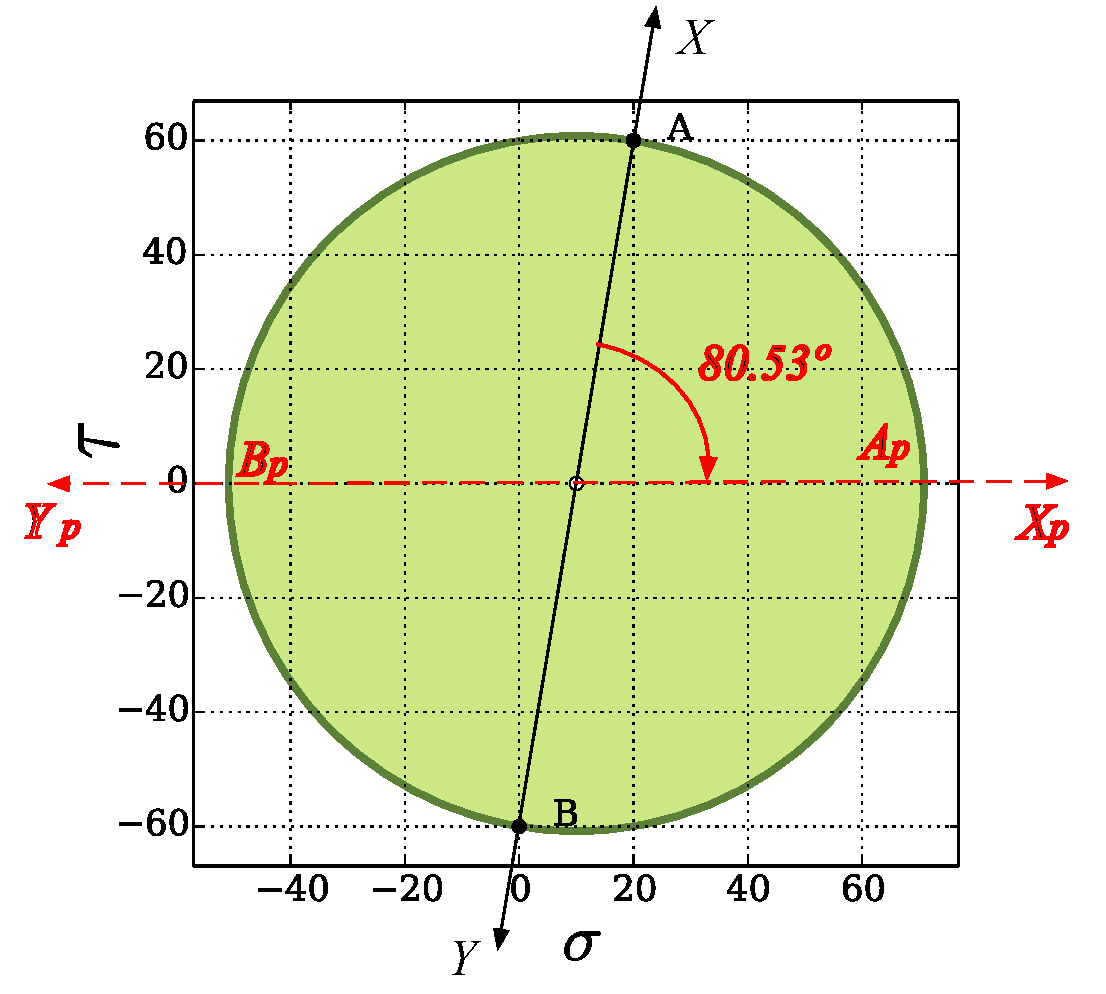
\includegraphics[width=2.8in]{TensorSup.pdf}\label{TensorSup}}
		\hspace{0.5cm}
		\subfloat [Cubo de tensiones]{ 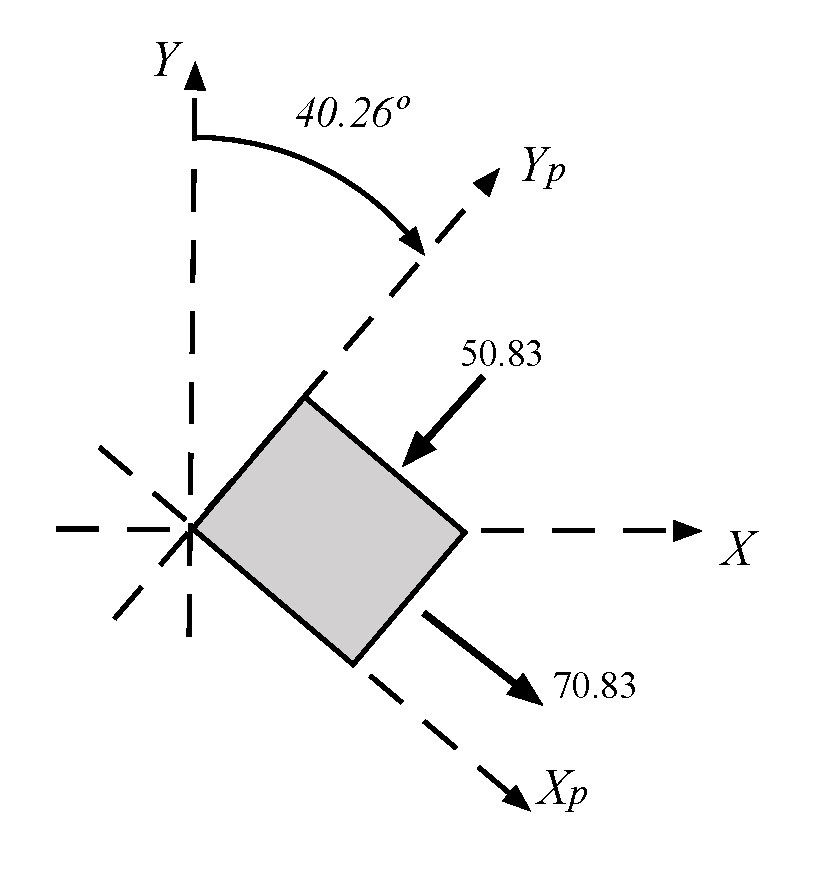
\includegraphics[width=2.8in]{CuboSup.pdf}\label{CuboSup}}		
	\caption{Estado de tension principal superpuesto }
	\label{TensSupPrin}
\end{figure}
%
El tensor escrito en direcciones principales es: 
\begin{equation}
 [\sigma^p_{2}] =
 	\begin{bmatrix}
     	70.83 & 0.0 &  \\
     	0.0 & -50.83 \\
 	\end{bmatrix}
\end{equation}

\end{enumerate}
%%%%
%%%%%

\subsubsection*{Ejemplo 3: Planos de falla}
Un punto material en un medio continuo est\'a sometido al estado de tensiones mostrado en la \cref{punto}. Si las líneas punteadas corresponden a planos de falla del material y sabiendo que los dos planos {\bf son perpendiculares entre sí}, se pide:

\begin{figure}[H]
	\centering
		\subfloat []{ 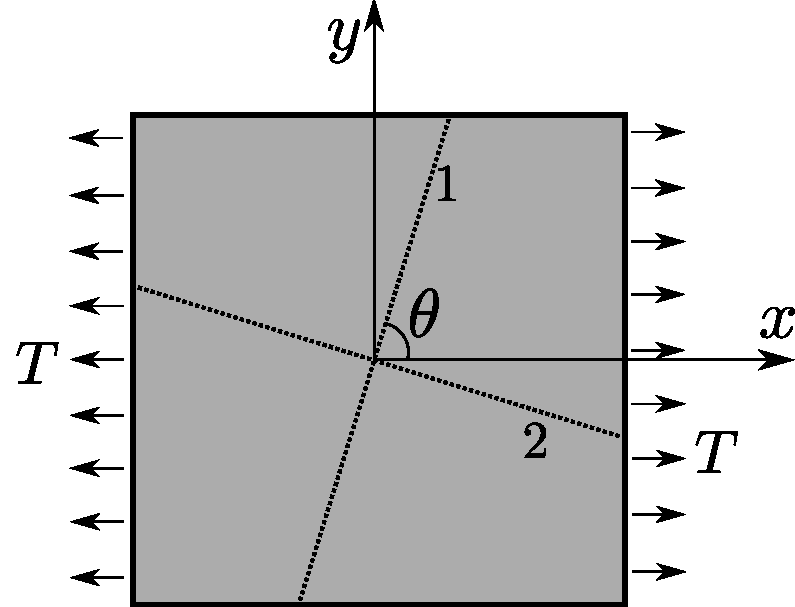
\includegraphics[width=2.8in]{punto.pdf}\label{punto}}		
	\caption{Estado de tensiones}
	\label{punto}
\end{figure}



\begin{itemize}

\item[•] Calcular las tensiones normal y tangencial al plano 1.

\textbf{Solución:}\\\\

Escribiendo el estado de tensiones como:

\begin{equation*}
[\sigma]
= 
\begin{bmatrix}
    T & 0 \\
    0 & 0
\end{bmatrix}
\end{equation*}

Para el plano 1 el vector normal es $\hat{n_1}=[ -\sin{\theta}, \cos{\theta} ]$, y la tensi\'on en el plano se calcula como:

\begin{equation*}
t_1 = [\sigma]\hat{n_1}
= 
\begin{bmatrix}
    T & 0 \\
    0 & 0
\end{bmatrix}
\begin{bmatrix}
   -\sin{\theta} \\
    \cos{\theta} \\
\end{bmatrix} \\
\end{equation*}

\begin{equation*}
t_1 = 
\begin{bmatrix}
    -T\sin{\theta} \\
    0 
\end{bmatrix} \\
\end{equation*}

La tensión normal se calcula proyectando la tensión $t_1$ sobre el vector $\hat{n_1}$, 

\begin{equation*}
\sigma_n = 
t_1 \cdot \hat{n_1} = 
\begin{bmatrix}
    -T\sin{\theta} \\
    0 
\end{bmatrix} \cdot
\begin{bmatrix}
    -\sin{\theta} \\
    \cos{\theta} 
\end{bmatrix} \equiv
T\sin^2\theta
\end{equation*}

El esfuerzo tangencial se puede calcular proyectando la tensión $t_1$ sobre un vector unitario inscrito en el plano 1. Dando como resultado:

\begin{equation*}
\tau = T\sin{\theta}\cos{\theta} 
\end{equation*}

\item[•] Calcular las tensiones normal y tangencial al plano 2.

\textbf{Solución:}\\\\

Siguiendo un proceso análogo al anterior, se llega a los siguientes resultados:

\begin{equation*}
\sigma_n = T\cos^2\theta 
\end{equation*}

\begin{equation*}
\tau = T\sin{\theta}\cos{\theta}
\end{equation*}

\item[•] Suponiendo que la falla va a ocurrir en alguno o en ambos planos, y que el material es infinitamente resistente a esfuerzos normales, pero no soporta esfuerzos cortantes mayores a $\tau_{adm} = T/4$, calcule el ángulo $\theta$ al cual se produce la falla e indique en cuál plano se presenta la misma. 

\textbf{Solución:}\\\\

\begin{figure}[h]
	\centering
	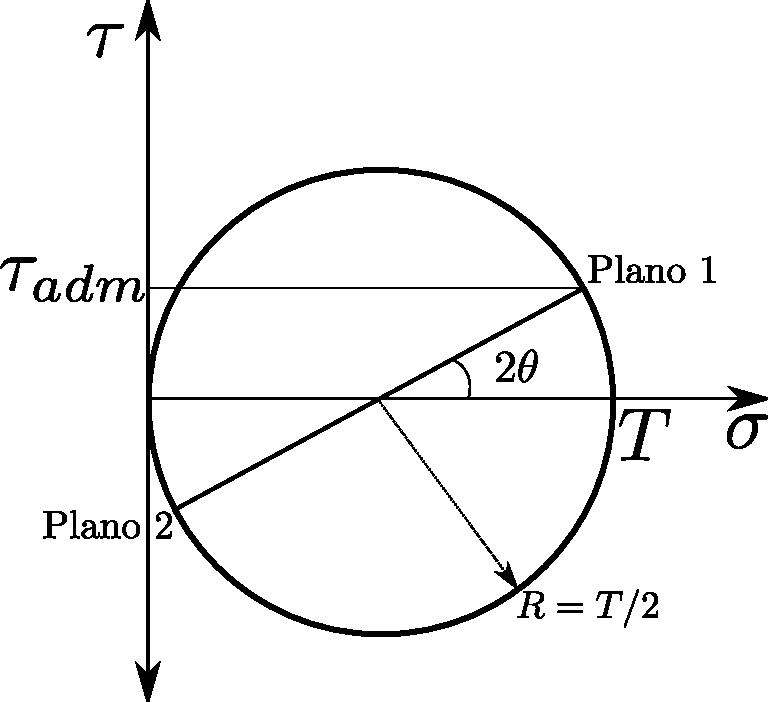
\includegraphics[width=8cm]{sol.pdf} 
	\caption{Circulo de Mohr correspondiente al Estado de tensiones de la \cref{punto}}
	\label{sol}
\end{figure}

Graficando el estado de tensiones como un círculo de Mohr (\cref{sol}), se ubica $\tau_{adm} = T/4$. Luego se llega a la relación:

\begin{equation*}
\sin{2\theta} = \frac{T/4}{T/2} = \frac{1}{2} \rightarrow
\theta = \frac{\pi}{12}
\end{equation*}

La falla se da en cualquier plano, ya que el valor del cortante es igual es ambos por ser perpendiculares.

\end{itemize}


\subsection*{Ejemplo 4: Refuerzo}

Un punto material de un medio continuo se encuentra sometido al estado de tensiones correpondiente al círculo de Mohr de la \cref{estado} y en el cual  $\tau_R$ es la resistencia al corte del material.

\begin{figure}[h]
	\centering
	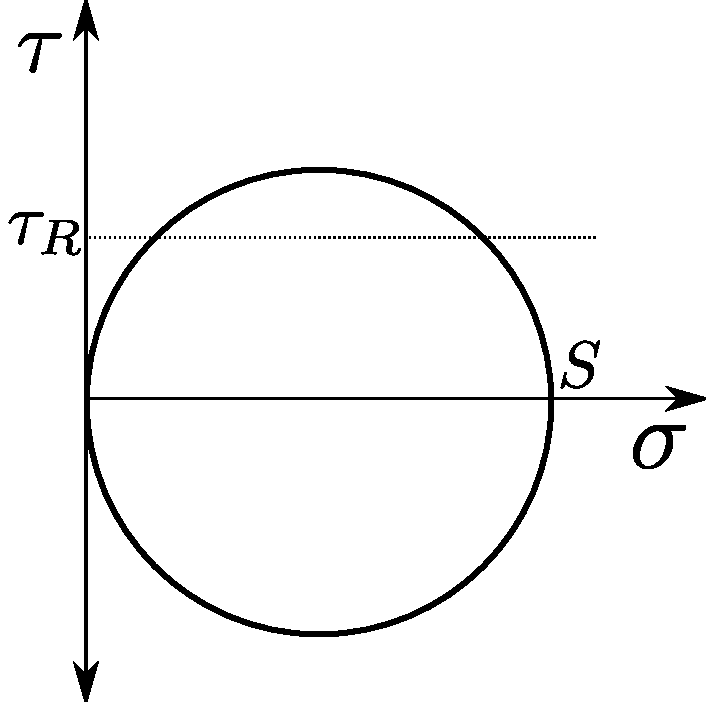
\includegraphics[width=7cm]{estado.pdf} 
	\caption{Estado de tensiones}
	\label{estado}
\end{figure}

Si se requiere aplicar una tracción $S = 3\tau_R$,  proponga una medida de mejoramiento del material, en términos de una aplicación adicional de tensiones, que garantice que éste no falle por cortante.

Del círculo de Mohr, se puede ver que la única manera de evitar que el material falle, es llevándolo a un estado de esfuerzos que no alcance $\tau_R$. En otras palabras, se necesita reducir el radio del círculo de Mohr. La reducción de radio necesaria se muestra en la \cref{modif}. 


\begin{figure}[H]
	\centering
		\subfloat []{ 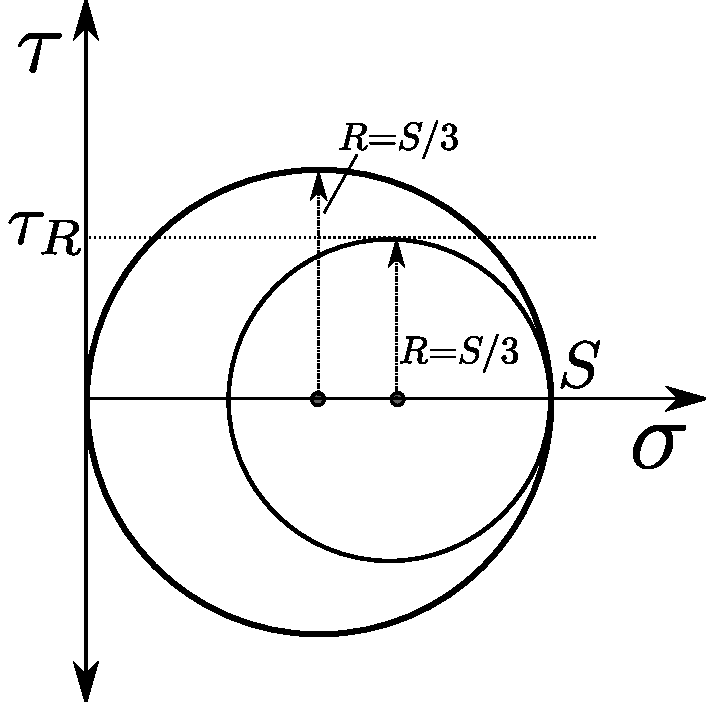
\includegraphics[width=2.8in]{cirmodif.pdf}\label{modif}}		
	\caption{Cambio en el estado de tensiones}
	\label{modif}
\end{figure}

De la \cref{modif} se ve el radio inicial $R=S/2$. El radio del nuevo círculo debe ser $R=S/3$ para que el material no falle por cortante. Entonces


\begin{equation*}
R = \frac{S}{3} =  \frac{\sigma_{xx} - \sigma_{yy}}{2} \rightarrow
\sigma_{yy} = \frac{S}{3}
\end{equation*}

\begin{figure}[h]
	\centering
	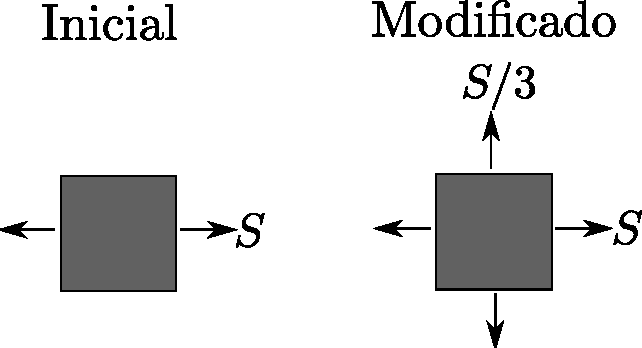
\includegraphics[width=7cm]{estado3.pdf} 
	\caption{Cambio en el estado de tensiones}
	\label{estado3}
\end{figure}

En la \cref{estado3} se ilustra le cambio en las configuraciones de tensiones.






\subsection*{Ejemplo 6: cálculo de valores principales}
%\footnote{Este ejemplo ha sido implementado en el siguiente notebook de Python http://nbviewer.ipython.org/urls/dl.dropbox.com/s/0bnyl2qvauk85i2/Ej4\_Eingen.ipynb}
Consideremos el siguiente estado de tensiones con componentes correspondientes a un sistema de referencia $x-y-z$;

\[\sigma  = \left[ {\begin{array}{*{20}{c}}
{200}&{100}&{300}\\
{100}&0&0\\
{300}&0&0
\end{array}} \right].\]

Se pide determinar las tensiones principales y sus direcciones asociadas.

La ecuación característica esta dada por;

\[{{\tilde \sigma }^3} - 200{{\tilde \sigma }^2} - 100000\tilde \sigma  = 0\]

donde identificamos los 3 invariantes como;


\[{I_\sigma } = 200\]
\[I{I_\sigma } =  - 100000\]
\[II{I_\sigma } = 0.\]
%
Resolviendo la ecuación característica determinamos las tensiones principales ${{\tilde \sigma }_1} = 432$, ${{\tilde \sigma }_2} = 0$ y ${{\tilde \sigma }_3} =  - 232$.

La dirección asociada con la tesion ${{\tilde \sigma }_1} = 432$ resulta de resolver;

\[\left[ {\begin{array}{*{20}{c}}
{ - 232}&{100}&{300}\\
{100}&{ - 432}&0\\
{300}&0&{ - 432}
\end{array}} \right]\left\{ {\begin{array}{*{20}{c}}
{{n_x}}\\
{{n_y}}\\
{{n_z}}
\end{array}} \right\} = \left\{ {\begin{array}{*{20}{c}}
0\\
0\\
0
\end{array}} \right\}\]

y

\[n_x^2 + n_y^2 + n_z^2 = 1.\]

De la segunda y tercera ecuación se tiene;

\[{n_y} = \frac{{100}}{{432}}{n_x}\]

y

\[{n_z} = \frac{{300}}{{432}}{n_x}.\]

Usando estas en $n_x^2 + n_y^2 + n_z^2 = 1$ se tiene que;

\[{n_x} =  \pm 0.807\]

mientras que ${n_y} = 0.187$ y ${n_z} = 0.560$. Por lo tanto la dirección asociada con la tensión principal ${{\tilde \sigma }_1} = 432$ corresponde al vector ${{\hat n}^1} = 0.807\hat i + 0.187\hat j + 0.560\hat k$.

Similarmente, resolviendo para ${{\tilde \sigma }_2} = 0$ se tiene;


\[\left[ {\begin{array}{*{20}{c}}
{ 200}&{100}&{300}\\
{100}&{ 0}&0\\
{300}&0&{0}
\end{array}} \right]\left\{ {\begin{array}{*{20}{c}}
{{n_x}}\\
{{n_y}}\\
{{n_z}}
\end{array}} \right\} = \left\{ {\begin{array}{*{20}{c}}
0\\
0\\
0
\end{array}} \right\}\]

De la segunda (o la tercera) ${n_x} = 0$ mientras que de la primera ${n_y} =  - 3{n_z}$. Finalmente de la condición $n_x^2 + n_y^2 + n_z^2 = 1$ se tiene que la dirección asociada con la tensión principal ${{\tilde \sigma }_2} = 0$ corresponde a ${{\hat n}^2} =-948\hat j + 0.316\hat k$.

Finalmente para la tensión principal ${{\tilde \sigma }_3} =  - 232$ resolvemos;

\[\left[ {\begin{array}{*{20}{c}}
{ 432}&{100}&{300}\\
{100}&{ 232}&0\\
{300}&0&{232}
\end{array}} \right]\left\{ {\begin{array}{*{20}{c}}
{{n_x}}\\
{{n_y}}\\
{{n_z}}
\end{array}} \right\} = \left\{ {\begin{array}{*{20}{c}}
0\\
0\\
0
\end{array}} \right\}.\]

De la segunda y la tercera se tiene que ${n_y} =  - \frac{{100}}{{231}}{n_x}$ y ${n_z} =  - \frac{{300}}{{231}}{n_x}$  mientras que de la condición $n_x^2 + n_y^2 + n_z^2 = 1$ se tiene que la dirección asociada con la tensión principal ${{\tilde \sigma }_3} = -232$ corresponde a ${{\hat n}^3} = 0.592\hat i - 0.255\hat j - 0.766\hat k$.

Nótese que en el paso final del cálculo de las direcciones principales ${{\hat n}^1}$, ${{\hat n}^2}$ y ${{\hat n}^3}$ se uso la condicíon $n_x^2 + n_y^2 + n_z^2 = 1$ para determinar una de las componentes a partir de las cuales era posible determinar las 2 restantes.

Por ejemplo en el caso de ${{\tilde \sigma }_1} = 432$ esta condición arrojó como resultado ${n_x} =  \pm 0.807$. Para determinar las componentes ${n_y}$ y ${n_z}$ usamos las relaciones ${n_y} = \pm \frac{{100}}{{432}}{n_x}$ y ${n_z} = \pm \frac{{300}}{{432}}{n_x}$ sobre las cuales trasladamos los 2 posibles signos de ${n_x}$. Lo anterior indica que las direcciones principales corresponden a vectores con direcciones opuestas lo cual es equivalente a observar de manera simultanea las tracciones sobre la dirección positiva y negativa del punto material. Por ejemplo, en el caso de la tensión principal ${{\tilde \sigma }_1} = 432$ obtenemos las direcciones ${{\hat n}^1} = 0.807\hat i + 0.187\hat j + 0.560\hat k$ y su opuesta ${{-\hat n}^1} = -0.807\hat i - 0.187\hat j - 0.560\hat k$.


\section*{Ejercicios}

\begin{enumerate}


\item \label{punto02} Las componentes del tensor de tensiones es un punto $P$
son:
		\[{[\sigma]} = \left[ \begin{array}{ccc}
		1 & 2 & 3 \\ 
		2 & 4 & 6 \\ 
		3 & 6 & 1
		\end{array}  \right] \enspace\]
%
Encontrar:
%
\begin{enumerate}
	\item El vector de tracci\'on $\mathbf{t}$ en $P$ para un plano normal al eje $x_1$;
	\item El vector de tracci\'on $\mathbf{t}$ en $P$ para un plano cuya normal es $\frac{1}{\sqrt{6}}(1,-1,2)$;
	\item El vector de tracci\'on $\mathbf{t}$ en $P$ para el plano $2x_1 - 2x_2 - x_3 = 0$;
\end{enumerate}

\item \label{punto03} La  \cref{planos} muestra dos estados de tensiones
para el mismo punto de un medio continuo. {Tomado del problema 4.8 en Reddy, J.N (2010). An introduction to continuum mechanics}
%
\begin{figure}[H]
	\centering
	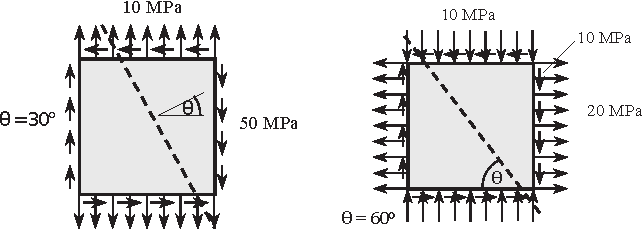
\includegraphics[width=12cm]{Ejer3_3.pdf}
	\caption{Estado de tensiones en un punto.}
	\label{planos}
\end{figure}
	%
\begin{enumerate}
	\item Determinar los esfuerzos normales sobre los planos mostrados con linea punteada en las figuras para cada uno de los estados.
	\item Determinar los esfuerzos cortantes sobre los planos mostrados con linea punteada en las figuras para cada uno de los estados.
	\item Para cada uno de los estados de tensiones mostrados determinar los valores propios y las direcciones principales.
	\item Asuma que ambos estados de tensiones ocurren al mismo tiempo y determine las direcciones principales y valores propios para el estado de tensiones resultantes.
	\item Para el estado de tensiones resultante de sumar los estados mostrados, determinar el estado de tensiones en un sistema de referencia que se encuentra a $90^0$ del mostrado en la figura.
	\item Para el estado de tensiones resultante de sumar los estados mostrados, determinar el estado de tensiones en un sistema de referencia que se encuentra a $180^0$ del mostrado en la figura.
	\item Para el estado de tensiones resultante de sumar los estados mostrados, determinar el estado de tensiones en un sistema de referencia que se encuentra a $270^0$ del mostrado en la figura.
	\item Para el estado de tensiones resultante de sumar los estados mostrados, determinar el estado de tensiones en un sistema de referencia que se encuentra a $45^0$ del mostrado en la figura.
\end{enumerate}


% *************************** %
\item \label{punto05} En la  \cref{cuna:tensiones} se dan las tensiones
$\vec{t}_1$ y $\vec{t}_2$ en dos planos no perpendiculares:\\
%	
\begin{figure}[H]
	\centering
	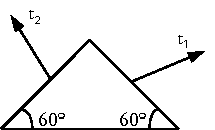
\includegraphics[width=6cm]{Ejer3_5.pdf}
	\caption{Estado de tensiones en un punto.}
	\label{cuna:tensiones}
\end{figure}
\begin{enumerate}
	\item Hallar el tensor de tensiones $[\sigma]$ en el sistema $x-y$ (horizontal y vertical), si \begin{large} $\vec{t}_1= 4 \hat{i} + 2 \sqrt{3} \hat{j}$ \end{large} y  \begin{large} $\vec{t}_2= -2 \hat{i} +0 \hat{j}$ \end{large}.\\
\end{enumerate}
%\newpage
\item \label{punto06} La \cref{direcc} muestra dos estados de tensiones
para el mismo punto de un medio continuo. 
%
\begin{figure}[H]
	\centering
	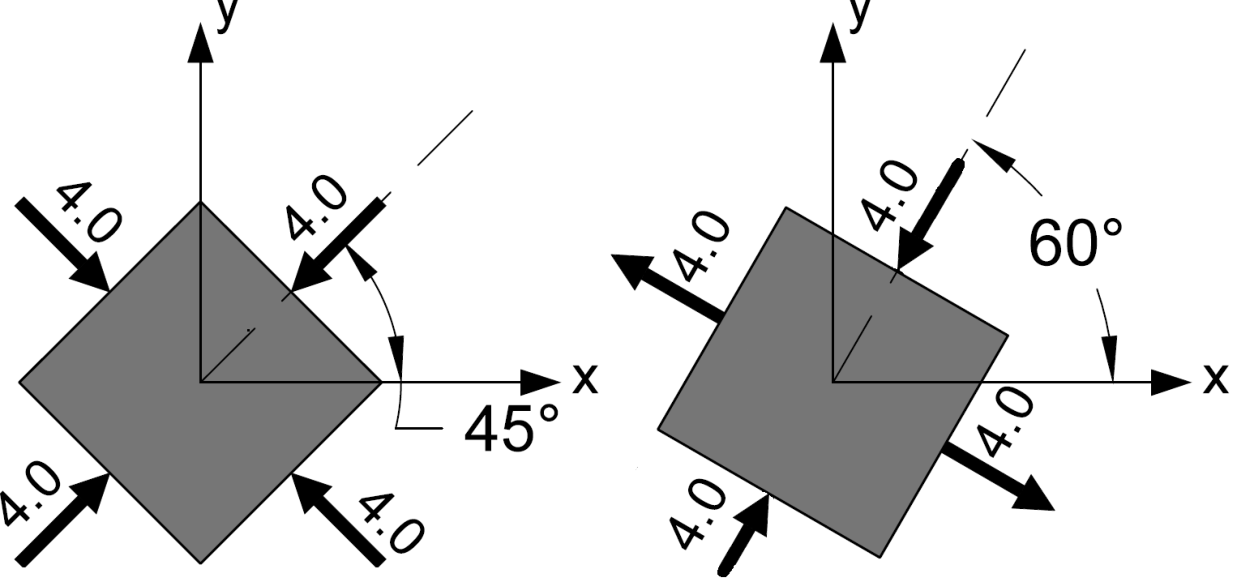
\includegraphics[width=9cm]{Ejer3_6.pdf}
	\caption{Estados de tensiones en un punto.}
	\label{direcc}
\end{figure}
%
\begin{enumerate}
	\item Para cada uno de los estados de tensiones mostrados determinar los
valores propios y las direcciones principales.
	\item Asuma que ambos estados de tensiones ocurren al mismo tiempo y determine
las direcciones principales y valores propios para el estado de tensiones resultantes.
	\item Para el estado de tensiones resultante de sumar los estados mostrados,
determinar el estado de tensiones en un sitema de referencia que se encuentra a $90^0$ del mostrado en la figura.
	\item Para el estado de tensiones resultante de sumar los estados mostrados,
determinar el estado de tensiones en un sitema de referencia que se encuentra a $180^0$ del mostrado en la figura.
	\item Para el estado de tensiones resultante de sumar los estados mostrados,
determinar el estado de tensiones en un sitema de referencia que se encuentra a $270^0$ del mostrado en la figura.
	\item Para el estado de tensiones resultante de sumar los estados mostrados,
determinar el estado de tensiones en un sitema de referencia que se encuentra a $45^0$ del mostrado en la figura.
\end{enumerate}
%
%\newpage
% *************************** %

% *************************** %
\item \label{punto08} Escribir el tensor de tensiones y hacer la
representaci\'on en el c\'irculo de Mohr para los siguientes caso:
%
\begin{enumerate}
	\item Caso unidimensional, estado de carga de tracci\'on.
	\item Caso unidimensional, estado de carga de compresi\'on.
	\item Caso bidimensional, estado de carga de tracci\'on.
	\item Caso bidimensional, estado de corte puro.
\end{enumerate}
% *************************** %

% *************************** %
\item \label{punto10} En la \cref{super:cuna-square} se dan las tensiones
para un mismo punto, estados I y II:  \footnote{Tomado del ejemplo 4.4 en Olivella, X; Saracíbar, C (2000). Mecánica de Medios Continuos para ingenieros}\\
%
\begin{figure}[H]
	\centering
	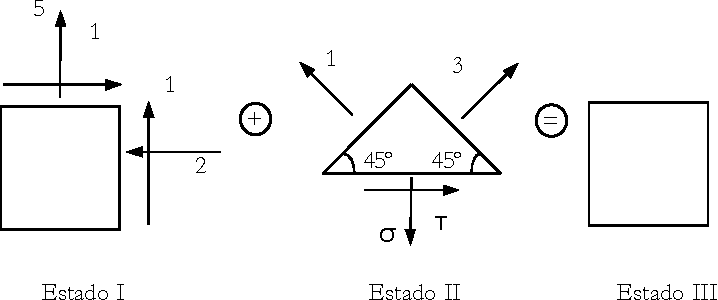
\includegraphics[width=11cm]{Ejer3_10.pdf}
	\caption{Estado de tensiones en un punto.}
	\label{super:cuna-square}
\end{figure}
%
\begin{enumerate}
	\item Hallar el estado de tensiones III si el estado I y II ocurren al mismo tiempo.
\end{enumerate}
% *************************** %
\item \label{punto11} La \cref{compresimple} corresponde al montaje
de la prueba de laboratorio de compresi\'on simple usada para determinar la resistencia del concreto.\\
%
\begin{figure}[H]	
	\centering	
	\subfloat [Ensayo de compresi\'on simple]{ 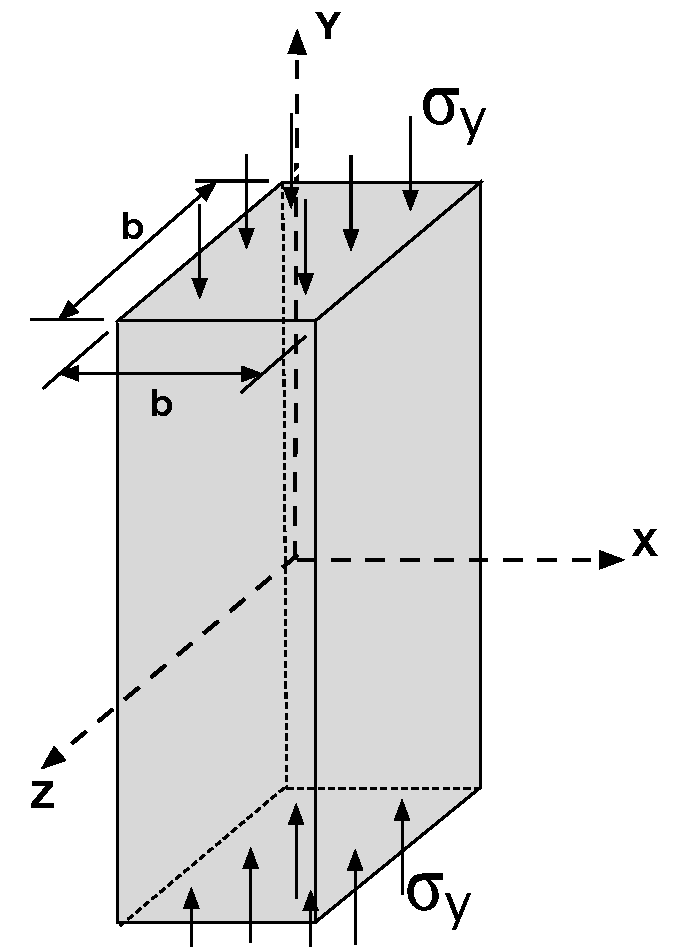
\includegraphics[width=2.8in]{Ejer3_11_1.pdf}\label{compresimple}}
	\hspace{10mm}
	\subfloat [Sección en planta de lado $b$, ensayo confinado]{ 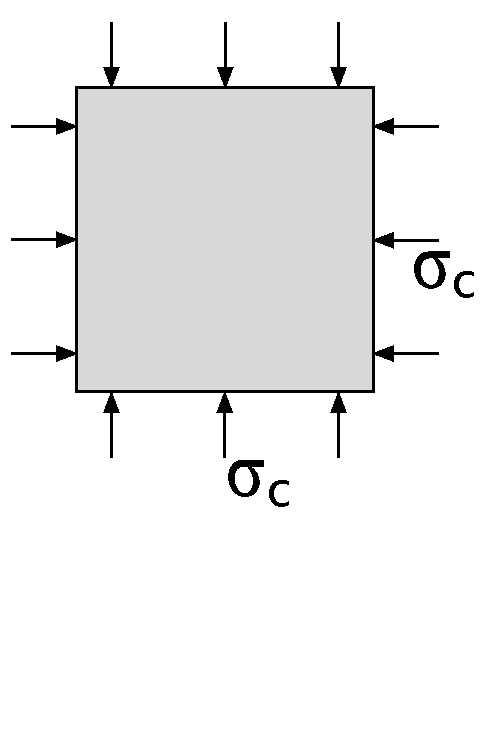
\includegraphics[width=2.0in]{Ejer3_11_2.pdf}\label{compreconf}}
	\caption{Columna en ensayo de compresión}
\end{figure}
%
\begin{enumerate}
	\item Hallar la tensión normal $\sigma_y$ m\'inima que produce la falla a cortante en el modelo presentado en la \cref{compresimple}, sabiendo que la capaciad m\'axima del material ante esfuerzos de corte es $\tau_{max}=A$.
	\item Chequear el equilibrio diferencial (local) de la probeta del ensayo.
	\item Si ahora se hace el mismo ensayo pero con confinamiento perimetral como el mostrado en la \cref{compreconf}, determine el valor minimo del esfuerzo de confinamiento $\sigma_c$ para obtener un un  esfuerzo axial máximo $\sigma_y = 10A$ y un cortante máximo  $\tau_{max}=A$.
\end{enumerate}

% *************************** %
%
% *************************** %
\item \label{punto13} La \cref{esta:tensiopoint} muestra el estado de
tensiones en un punto al interior de un Medio Continuo. Sobre la cara asociada al eje $y'$ se dan las tensiones $\sigma_{y'y'}$ y $\tau_{y'x'}$ y sobre la cara asociada al eje $x'$ se da el vector de tracciones expresado en el sistema de referencia $x-y$.\\
%
\begin{figure}[H]
	\centering
	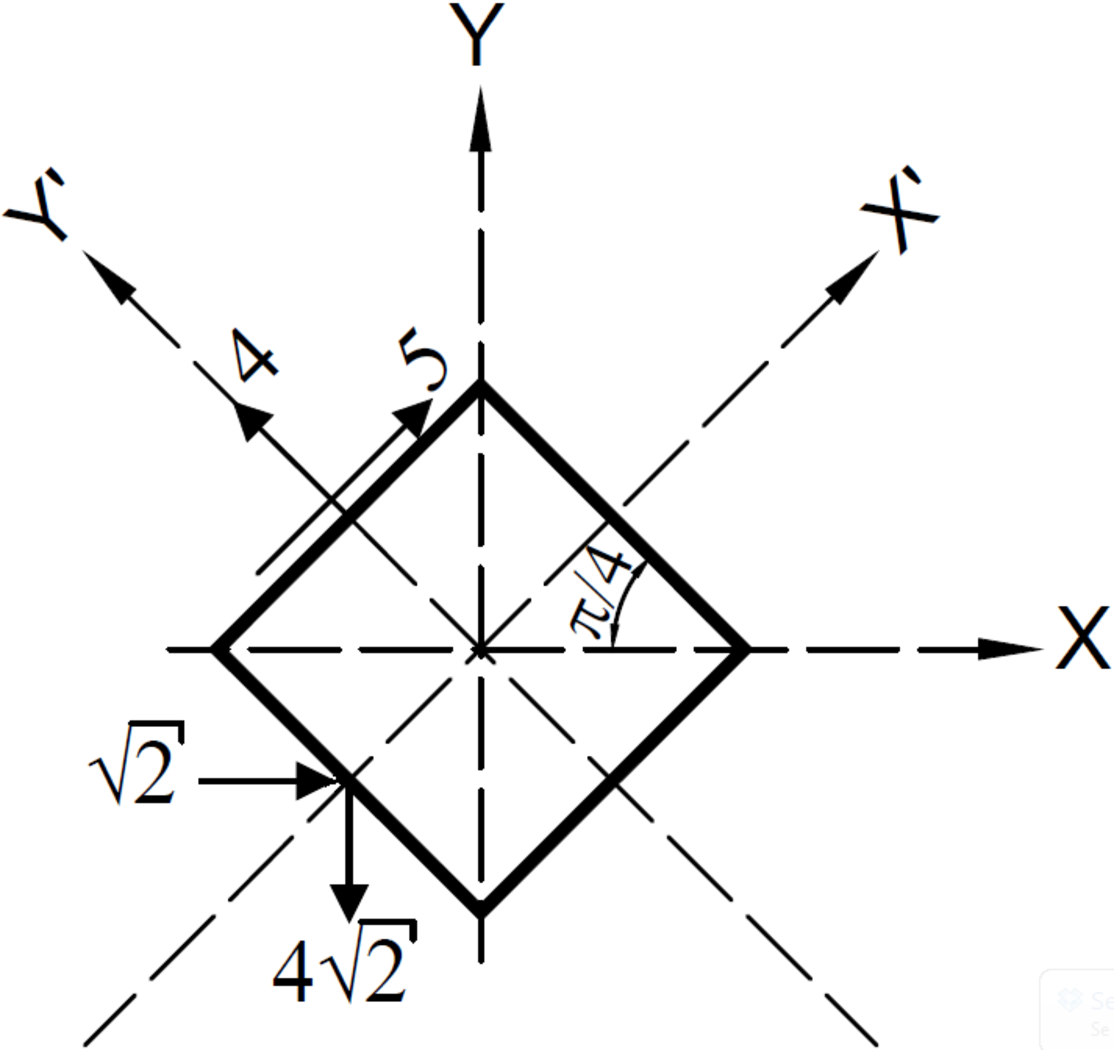
\includegraphics[height=6.25cm]{Ejer3_13.pdf}
	\caption{Estado de tensiones en un punto al interior de un medio continuo.}
	\label{esta:tensiopoint}
\end{figure}

\begin{enumerate}
	\item Escribir el tensor de tensiones en el sistema de referencia $x'-y'$.
	\item Escribir el tensor de tensiones en el sistema de referencia $x-y$.
\end{enumerate}
% *************************** %


\end{enumerate}

\end{document}
% ***** End *****


